\documentclass[letter,12pt]{article}
\usepackage{verbatim}
\usepackage[utf8]{inputenc}
\usepackage{graphicx}
\usepackage{mathrsfs}
\graphicspath{ {images/} }
\usepackage{amssymb,amsmath,amsthm, graphicx}  
\usepackage{hyperref}
\usepackage{mathtools}
\usepackage{xcolor}
\usepackage{caption}
\usepackage{subcaption} 
\usepackage{setspace}
\usepackage{url}
\usepackage{natbib}
\usepackage[utf8]{inputenc}
\usepackage[section]{algorithm}
\usepackage{algpseudocode}
\DeclareGraphicsExtensions{
	fig_RunData2_K2_init3.png,
	fig_RunData2_K5_init3.png,
	fig_RunData2_K10_init3.png}
\DeclareMathOperator*{\argmax}{arg\,max}
\newcommand*\rfrac[2]{{}^{#1}\!/_{#2}}
\setlength{\topmargin}{-.5in}
\setlength{\textheight}{9in}
\setlength{\oddsidemargin}{.125in}
\setlength{\textwidth}{6.25in}
\begin{document}
\title{SQP Methods for QN2 Quasi Newton Acceleration of the EM Algorithm}
\author{Final Project\\CSCI-GA.2945 Numerical Optimization\\Justin Mao-Jones\\New York University}
\renewcommand{\today}{December 14, 2014}
\maketitle

\section{Introduction}

In 1977, \citeauthor*{dempsterlr77} (henceforth abbreviated DLR) proposed the EM algorithm, which has since become, and continues to be, a popular method for computing maximum likelihood estimates from incomplete data.  \cite{wu1983} showed that under certain properties, the sequence of EM iterates converge to a unique maximum likelihood estimate.

A drawback of the EM algorithm is its tendency towards slow convergence.  In certain practical applications, the EM algorithm has been shown to exhibit sublinear convergence.  For examples see \cite{lange1995a,jamshidianj93,jamshidianj97}.

Modifications and extensions of the EM algorithm have been proposed to speed up convergence, and are often referred to as "accelerators".  In this project, I focus on the QN2 introduced by \cite{jamshidianj97}.  QN2 has been referred to as a Quasi Newton accelerator of the EM algorithm.  I explain the structure of the QN2 algorithm in relation to the underlying EM concepts and conventional Quasi Newton optimization concepts.  I then exhibit and discuss the results of an application of the QN2 algorithm to deriving MLE parameter estimates of a mixture of poissons.  \cite{jamshidianj97} applied QN2 to a mixture of 2 poissons.  I generalize this to a mixture of $n$ poissons.

For the sake of the interested reader, I include the major steps of the derivation of both EM and QN2 algorithms.  An additional goal of this project is to present QN2 in such a way that a reader familiar with Quasi Newton methods, but with little experience in either EM and QN2 could understand the underlying theory and implement both the EM and QN2 algorithms.

\section{EM Algorithm}

The EM algorithm, otherwise known as expectation-maximization, is a method for computing the maximum likelihood parameter estimates from incomplete data.  Incomplete data is a set of data in which some or all observations contain variables with missing data.  

To use an illustrative example, consider a set of $m$ randomly sampled observations $\{x_1,...,x_m\}$.  Suppose that we would like to explore the possibility that each of these observations comes from one of $n$ poisson-distributed populations with unknown parameters $\theta=(\gamma_1,...,\gamma_n,\lambda_1,...,\lambda_n)^T$, where $\gamma_r$ and $\lambda_r$ are the parameters of population $r$.  This construction is known as a mixture of poissons.  We seek to estimate $\theta$ using maximum likelihood.  We do not know which of the $n$ populations the observation $x_i$ corresponds to.  Let $z_i \in \{1,...,n\}$ denote the identity of the population that $x_i$ belongs to.  In this example, $\{x_1,...,x_m\}$ is incomplete data, $\{z_1,...,z_m\}$ is missing data, and $\{(x_1,z_1),...,(x_m,z_m)\}$ is the complete (unknown) data.

The probability distribution of an incomplete observation $x_i$ conditional on $z_i$ is:
\[
p(x_i=j|z_i=r,\theta) = \frac{e^{-\lambda_r}\lambda_r^{j}}{j!}  
\indent
\lambda_r \geq 0
\]
The probability distribution of the missing data is:
\[
p(z_i=r|\theta) = \gamma_r
\indent
\text{where}
\indent 
\sum_{r=1}^{n}\gamma_r = 1
\indent
\text{and}
\indent 
0 \leq \gamma_r \leq 1
\]
The probability distribution of the complete data is:
\begin{equation} \label{eq_constraint}
p(x_i=j,z_i=r|\theta) 
= p(x_i=j|z_i=r,\theta)p(z_i=r|\theta) = \gamma_r\frac{e^{-\lambda_r}\lambda_r^{j}}{j!}
\end{equation}
We wish to compute the maximum likelihood estimates, and so we begin with the log likelihood function, which is defined as:
\[
l(\theta) = \log(\prod_{i=1}^{m}p(x_i|\theta)) = \sum_{i=1}^{m} \log(p(x_i|\theta))
\]
This is the point at which a method such as the EM algorithm becomes useful.  Since $z_i$ are unobserved, solving for the roots of the derivative of $l(\theta)$ can be an intractable problem:
\[
\sum_{i=1}^{m} \log(p(x_i|\theta)) = \sum_{i=1}^{m} \log\left(\sum_{r=1}^{n}p(x_i,z_i|\theta))\right)
\]
Fortunately, $l(\theta)$ can be converted into a more manageable form.  Consider the probability distribution $p(\vec{z}|\vec{x},\phi)$.  Note that this function is parameterized by $\phi$ and not $\theta$.  Per the EM literature:
\[
l(\theta) = \log(p(\vec{x}|\theta)) 
= \int_{\vec{z}}p(\vec{z}|\vec{x},\phi)\log(p(\vec{x}|\theta))d\vec{z}
\]
\[
=
E[\log(p(\vec{x},\vec{z}|\theta))|\vec{x},\phi]
-
E[\log(p(\vec{z}|\vec{x},\theta))|\vec{x},\phi]
\]
\begin{equation} \label{eq:QH}
=Q(\theta|\phi)
-H(\theta|\phi)
\end{equation}

where $Q(\theta|\phi)$ and $H(\theta|\phi)$ are defined as the left and right conditional expectations, respectively.  In the words of \cite{lange1995a}, this derivation can seem "slightly mysterious."  In order to shed some light on this result, I will show how it follows from our specific mixture of poissons problem.  We will use the following identity, which follows from the assumption that our observations are independent:
\[
1 = \int_{\vec{z}}p(\vec{z}|\vec{x},\phi)d\vec{z}
= \prod_{j=1}^{m}\int_{z_j}p(z_j|x_j,\phi)dz_j
\]
The previous identity is true due to the identity $\int_{z_j}p(z_j|x_j,\phi)dz_j=1$.  Now, multiply $l(\theta)$ by $\int_{\vec{z}}p(\vec{z}|\vec{x},\vec{\phi})d\vec{z}=1$:
\[
l(\theta)
= \left( \sum_{i=1}^{m} \log(p(x_i|\theta)\right)
\prod_{j=1}^{m}\int_{z_j}p(z_j|x_j,\phi)dz_j
\]
\[
= \left( \sum_{i=1}^{m} \int p(z_i|x_i,\phi)\log(p(x_i|\theta)dz_i\right)
\prod_{j=1}^{m}\int_{z_j}p(z_j|x_j,\phi)dz_j
=\sum_{i=1}^{m} \int p(z_i|x_i,\phi)\log(p(x_i|\theta)dz_i
\]
The previous result was derived by putting the $i^{th}$ integral inside of the summation and the log inside of the integral.  Now we use Bayes' theorem to derive a useful result:
\[
\sum_{i=1}^{m} \int p(z_i|x_i,\phi)\log(p(x_i|\theta))dz_i
= \sum_{i=1}^{m} \int p(z_i|x_i,\phi) \log \left(p(x_i,z_i|\theta)\frac{p(x_i|\theta)}{p(x_i,z_i|\theta)}\right) dz_i
\]
\[
=
\sum_{i=1}^{m} \int p(z_i|x_i,\phi) \log \left(\frac{p(x_i,z_i|\theta)}{p(z_i|x_i,\theta)}\right) dz_i
\]
\[
=
\sum_{i=1}^{m} \int p(z_i|x_i,\phi) \log \left(p(x_i,z_i|\theta)\right) dz_i
-
\sum_{i=1}^{m} \int p(z_i|x_i,\phi) \log \left(p(z_i|x_i,\theta)\right) dz_i
\] 
\[
=Q(\theta|\phi)
-H(\theta|\phi)
\]
This result is useful, because $\nabla_{\theta}l(\theta)$ evaluated at $\theta = \phi$ makes $H(\theta|\phi)$ go to 0: 

\[
\nabla_{\theta}H(\theta|\phi)|_{\theta = \phi}
=
\nabla_{\theta}\sum_{i=1}^{m} \int p(z_i|x_i,\phi) \log \left(p(z_i|x_i,\theta)\right) dz_i
\]
\[
=
\sum_{i=1}^{m} 
\int p(z_i|x_i,\phi) 
\nabla_{\theta}|_{\theta = \phi}
\log \left(p(z_i|x_i,\theta)\right) dz_i
=
\sum_{i=1}^{m} 
\int \dfrac{p(z_i|x_i,\phi)}{p(z_i|x_i,\phi)} 
\nabla_{\theta}|_{\theta = \phi}
p(z_i|x_i,\theta) dz_i
\]
\[
=
\sum_{i=1}^{m} 
\nabla_{\theta}|_{\theta = \phi}
\int 
p(z_i|x_i,\theta) dz_i
=
\sum_{i=1}^{m} 
\nabla_{\theta}|_{\theta = \phi}
1
=0
\]
Thus, we have the following EM identity:
\begin{equation} \label{eq:dl_is_dq}
\nabla_{\theta}l(\theta)|_{\theta = \phi}
=
\nabla_{\theta}Q(\theta|\phi)|_{\theta = \phi}
\end{equation}
One way to think about this identity is that it shows where $\nabla_{\theta}l(\theta)|_{\theta = \phi}$ intersects with a more tractable function $\nabla_{\theta}Q(\theta|\phi)|_{\theta = \phi}$ in an extended parameter space.  The EM algorithm moves along this intersection in the hopes of finding a zero.

This brings us to the specific steps of the EM algorithm, which works as follows.  Given an iterate $\theta_k$, the next iterate $\theta_{k+1}$ is defined as the $\theta$ that maximizes $Q(\theta|\phi)$ where $\phi$ is set to $\theta_k$.
\[
\theta_{k+1} = \argmax_{\theta}  Q(\theta|\theta_k) = M(\theta_k)
\]
The function $M(\theta_k)$ is known as the EM operator.  The algorithm begins with an initial parameter set $\theta_0$ and terminates when either $|M(\theta_k)-\theta_k|$ is small enough or a maximum number of iterations has been reached.


\begin{algorithm}
\caption{Expectation-Maximization}
\label{alg:em}
\begin{algorithmic}[1]
\State Initialize $\theta_0$; Define \textbf{maxit}, \textbf{ftol}
\State $k = 0$
\While{$|M(\theta_k)-\theta_k|<$ \textbf{ftol}
and $k < $ \textbf{maxit}}
\State $k = k+1$
\State $\theta_{k+1} = M(\theta_k)$
\EndWhile
\end{algorithmic}
\end{algorithm}

\subsection{Convergence} \label{section:convergence}

\cite{wu1983} identified several key convergence properties of the EM algorithm.  The relevant one here is:
\begin{list}{-}{}
\item "If the unobserved complete-data specification of the can by defined by a curved exponential family with compact parameter space, all the limit points of any EM sequence are stationary points of the likelihood function."
\item It cannot be guaranteed that EM converges to the maximum likelihood estimator.
\item It cannot be guaranteed that a stationary point is a local maximum.
\end{list}

Mixtures of Poissons are within the exponential family, and thus we can assume that the EM algorithm will converge to a stationary point.  Furthermore, since we are working with probabilities, the maximum likelihood function is bounded above by 1. 

Note we do not have enough information about the likelihood function of the mixture of Poissons to determine whether or not we converge to the MLE or even a local maximum.  Thus, in the Comparison section below, I discuss results in terms of convergence to stationary points.

\section{QN2 Algorithm}

The QN2 Algorithm by \cite{jamshidianj97} is described as a Quasi Newton method using Broyden-Fletcher-Goldfarb-Shanno (BFGS) symmetric rank 2 updating.  I will show how it can be applied with Sequential Quadratic Programming to estimate n-dimensional mixture models with equality constraints.   

To begin, we define the following:
\begin{equation} \label{eq:define_g}
g(\theta_k) = \nabla_{\theta}Q(\theta|\phi)|_{\theta =\theta_k, \phi = \theta_k}
= \nabla_{\theta}Q(\theta_k|\theta_k)
\end{equation}
\begin{equation} \label{eq:define_gsquiggly}
\tilde{g}(\theta_k) = M(\theta_k) - \theta_k
\end{equation}
The first function $g(\theta_k)$ is the gradient of $Q$ with respect to $\theta$ evaluated at $\theta = \theta_k$ and $\phi=\theta_k$.  To simplify notation, I re-write this as $\nabla_{\theta}Q(\theta_k|\theta_k)$.  Note that we will never take a derivative with respect to $\phi$ The second function is the would-be step size of the EM operator $M$.   

\cite{jamshidianj93} showed the following property of the EM step:
\begin{equation} \label{eq:ddq_approx}
\tilde{g}(\theta_k) \approx -(\nabla^2_{\theta}Q(\hat{\theta}|\hat{\theta}))^{-1}g(\theta_k)
\end{equation}
where $\nabla^2_{\theta}Q$ is the Hessian of $Q$ and $\hat{\theta}$ is a local maximum of $l(\theta)$.  

We are using a Quasi Newton method, and so would like to approximate  $(\nabla^2_{\theta}l(\theta))^{-1}$, the inverse Hessian of the log likelihood function, 
\[
(\nabla^2_{\theta}l(\theta))^{-1}
=
(\nabla^2_{\theta}Q(\theta|\phi)
-
\nabla^2_{\theta}H(\theta|\phi))^{-1}
\]
which, using equations (\ref{eq:QH}) and (\ref{eq:ddq_approx}), can be approximated as follows:
\[
(\nabla^2_{\theta}l(\theta))^{-1}g(\theta)
\approx
-\tilde{g}(\theta)
+
Sg(\theta)
\]
where we define $S$ as a Quasi-Newton approximation to
\[
(\nabla^2_{\theta}l(\theta))^{-1}-(\nabla^2_{\theta}Q(\hat{\theta}|\hat{\theta}))^{-1}
\]
This approximation will be used to define the Quasi-Newton update step.  Notice that this is a modification to the conventional Quasi-Newton method, because it contains a floating inverse Hessian approximation of $Q(\hat{\theta}|\hat{\theta})$.  The presumption here is that this floating value should aid the overall approximation of the inverse Hessian of the log likelihood, and thus speed up convergence.

The resulting update step to $\theta_k$ defined below and assumes a line search methodology is used to determine $\alpha_k$, which is described in the next section.  For ease of reading, I make abbreviations such as $g_k = g(\theta_k)$.
\[
\theta_{k+1} = \theta_k - \alpha_k d_k
\indent
\text{where}
\indent
d_k = \tilde{g}_k(\theta_k) - S_kg(\theta_k)
\]
NOTE: \cite{jamshidianj97} p.575 contains an error in step a, which incorrectly defines $d_k=-\tilde{g}_k(\theta_k) + S_kg(\theta_k)$.

\cite{jamshidianj97} point out that $d_k$ can be viewed as a modification to the EM step, which is why they label QN2 as an EM accelerator.

The BFGS update is then derived as follows.  Using the notation used by \cite{jamshidianj97}, define:
\[
\begin{array}{l}
\Delta \tilde{g}_k = \tilde{g}_{k+1} - \tilde{g}_{k} \\
\Delta g_k = g_{k+1} - g_k
\end{array}
\]
The classic BFGS update of the inverse Hessian is (see \cite{nocedalwright_BFGS}, p. 136-140):
\[
H_{k+1} = (I - \frac{\Delta \theta_k\Delta g_k^T}{\Delta g_k^T\Delta \theta_k})H_k(I-\frac{\Delta g_k\Delta \theta_k^T}{\Delta g_k^T\Delta \theta_k})+\frac{\Delta \theta_k\Delta \theta_k^T}{\Delta g_k^T\Delta \theta_k}
\]
\[
= H_k - H_k\frac{\Delta g_k\Delta \theta_k^T}{\Delta g_k^T\Delta \theta_k} - \frac{\Delta \theta_k\Delta g_k^T}{\Delta g_k^T\Delta \theta_k}H_k + \frac{\Delta \theta_k\Delta g_k^TH_k\Delta g_k\Delta \theta_k^T}{(\Delta g_k^T\Delta \theta_k)^2}+\frac{\Delta \theta_k\Delta \theta_k^T}{\Delta g_k^T\Delta \theta_k}
\]
Thus,
\[
\Delta H_k = H_{k+1} - H_k
= (1+\frac{\Delta g_k^TH_k\Delta g_k}{\Delta g_k^T\Delta \theta_k})\frac{\Delta \theta_k\Delta \theta_k^T}{\Delta g_k^T\Delta \theta_k} - \frac{\Delta \theta_k\Delta g_k^TH_k + (\Delta \theta_k\Delta g_k^TH_k)^T}{\Delta g_k^T\Delta \theta_k}
\]
If we construct the inverse Hessian approximation as
\[
H_k = (\nabla^2_{\theta}Q(\hat{\theta}|\hat{\theta}))^{-1} + S_k
\]
then, using Eqn (\ref{eq:ddq_approx}), it follows that
\[\begin{array}{c}
H_k  g_k =  -\tilde{g}_k + S_kg_k
\\
H_k  g_{k+1} = -\tilde{g}_{k+1} + S_kg_k
\\
H_k \Delta g_k = -\Delta \tilde{g}_k + S_k\Delta g_k
\end{array}\
\]
The QN2 BFGS update step is:
\begin{equation} \label{eq:BFGS}
\Delta S_k = H_{k+1} - H_k =
\left(
1 + \frac{\Delta g_k^T \Delta \theta_k^*}{\Delta g_k^T \Delta \theta}
\right)
\frac{\Delta \theta_k \Delta \theta_k^T}{\Delta g_k^T \Delta \theta_k}
-
\frac{\Delta \theta_k^* \Delta \theta_k^T + (\Delta \theta_k^* \Delta \theta_k^T)^T}{\Delta g_k^T \Delta \theta_k}
\end{equation}
where
\[
\Delta \theta_k^* = -\Delta \tilde{g_k} + S_k \Delta g_k
\]
As will be seen in the next section, it is important to initialize $S_0$ to $\boldsymbol{0}$.

\subsection{Constraints}
The problem of finding the maximum likelihood estimate is often a constrained optimization problem.  For example, in the mixture of poissons, we have the following constraints:
\[
(\lambda_k)_r \geq 0 \indent \indent
0 \leq (\gamma_k)_r \leq 1 \indent \indent
r \in \{1,...,n\}
\]
\begin{equation} \label{eqn:equalityconstraint}
\sum_{r=1}^{n} (\gamma_k)_r = 1
\end{equation}

Here $(\lambda_k)_r$ and $(\gamma_k)_r$ are defined as the $\lambda$ and $\gamma$ parameters, respectively, of population $r$ at iteration $k$.  While I have not performed an exhaustive literature search, it seems there is a tendency in the literature to ignore all but the equality constraint.  The presumption then must be that in practical problems, the maximum likelihood estimate exists strictly inside the feasible region.  

In the mixture of poissons example, this would make sense.  $(\lambda_k)_r=0$ would require that all observations have value $0$, and thus maximum likelihood estimation would not be useful.  $(\gamma_k)_r$ cannot become zero, because, as will be shown later, the derivative would go to infinity.  Similarly, $(\gamma_k)_r$ cannot become $1$ either, since a value of $1$ in any $(\gamma_k)_r$ would imply a zero in the other $\gamma$'s.

In order to enforce the inequality parameter constraints, we use the following pseudo line search method:
 

\begin{algorithm}
\caption{Constraint Enforcement}
\label{alg:constraint_enforecement}
\begin{algorithmic}[1]
\State Given $\theta_k$, $d_k$
\State $\alpha_k = 1$
\While{$\theta_k + \alpha_k d_k$ violates constraints}
\State $\alpha_k = \alpha_k / 2$
\EndWhile
\State return $\alpha_k$
\end{algorithmic}
\end{algorithm}

The equality parameter constraint can be handled by appropriate initialization of $\theta_0$ and $S_0$.  To explain why, consider that at iteration $k$, we assume the relationship $\sum_{r=1}^{n}[\gamma_{k}]_r=1$ holds.  Then, in order for Eqn (\ref{eqn:equalityconstraint}) to be satisfied at each successive iteration $k+1$, the step along the $\gamma$ parameters $\Delta \gamma_k = \gamma_{k+1} - \gamma_k = \alpha_k(d_k)_{\gamma}$ must satisfy the relationship
\begin{equation} \label{eq:gammastepzero}
\sum_{r=1}^{n} [\Delta \gamma_k]_r
=
\sum_{r=1}^{n}[\gamma_{k+1}]_r - [\gamma_k]_r
= 0
\end{equation}
Thus, $\sum_{r=1}^{n}[\gamma_{k+1}]_r=1$ if and only if $\sum_{r=1}^{n} [\Delta \gamma_k]_r = 0$.  In order for this to be true, it must be true that:
\begin{equation} \label{eq:dstepzero}
\sum_{r=1}^{n} [(d_k)_{\gamma}]_r
=
\sum_{r=1}^{n} [(\tilde{g}_k)_{\gamma}]_r - [(S_kg_k)_{\gamma}]_r = 0
\end{equation}
First, assume that the following is true for $S_{k}$ and any vector $v \in \Re^{2n}$:
\begin{equation} \label{eqn:Sgzero}
\sum_{r=1}^{n} [(S_{k}v)_{\gamma}]_r = 0
\end{equation}
Second, consider $\sum_{r=1}^{n} [(\tilde{g}_k)_{\gamma}]_r$:
\begin{equation} \label{eq:gsquigglyzero}
\sum_{r=1}^{n} [(\tilde{g}_k)_{\gamma}]_r
=
\sum_{r=1}^{n} [(M(\theta_k) - \theta_k)_{\gamma}]_r
=
\sum_{r=1}^{n} [(M(\theta_k))_{\gamma}]_r - \sum_{r=1}^{n} [\gamma_k]_r = 1 - 1 = 0
\end{equation}
which holds true for all $k$.  By definition, $M(\theta_k)$ is another estimate of $\theta$ that satisfies all parameter constraints.  An explicit example of $M(\theta_k)$ is provided in Section \ref{section:poisson}

By assumption (\ref{eqn:Sgzero}) and Eqn (\ref{eq:gsquigglyzero}), Eqn (\ref{eq:dstepzero}) holds true, and thus Eqn (\ref{eq:gammastepzero}) holds for $k$.  However, this does not yet prove that Eqn (\ref{eq:gammastepzero}) will hold for iteration $k+1$ or any other subsequent iterations.  

Thus, now we need to show that:
\begin{equation} \label{eq:dpluszero}
\sum_{r=1}^{n} [(d_{k+1})_{\gamma}]_r
=
\sum_{r=1}^{n} [(\tilde{g}_{k+1})_{\gamma}]_r - [(S_{k+1}g_{k+1})_{\gamma}]_r = 0
\end{equation}
Eqn (\ref{eq:gsquigglyzero}) implies that:
\[
\sum_{r=1}^{n} [(\tilde{g}_{k+1})_{\gamma}]_r = 0
\]
And so all that is left is to show that:
\[
0 = \sum_{r=1}^{n} [(S_{k+1}g_{k+1})_{\gamma}]_r 
= \sum_{r=1}^{n} [((S_{k}+\Delta S_k)g_{k+1})_{\gamma}]_r
=\sum_{r=1}^{n} [(S_{k}g_{k+1})_{\gamma}]_r
+\sum_{r=1}^{n} [(\Delta S_kg_{k+1})_{\gamma}]_r
\]
By the assumption in Eqn (\ref{eqn:Sgzero}), we already have that $\sum_{r=1}^{n} [(S_{k}g_{k+1})_{\gamma}]_r=0$.  Thus, to show that $\sum_{r=1}^{n} [(\Delta S_kg_{k+1})_{\gamma}]_r=0$, we need to evaluate the BFGS update, which has three matrix terms: $\Delta \theta_k \Delta \theta_k^T, \Delta \theta_k \Delta {\theta_k^*}^T,$ and $\Delta \theta_k^* \Delta \theta_k^T$.  Consider any vector $u \in \Re^{2n}$
\[
\Delta \theta_k\Delta \theta_k^Tu = 
\left[
\begin{array}{cc}
\Delta \gamma_k 
\\
\Delta \lambda_k 
\end{array}
\right]
\Delta \theta_k^Tu
\indent
\text{which implies}
\indent
\sum_{r=1}^{n} [(\Delta \theta_k\Delta \theta_k^Tu)_{\gamma}]_r 
=
\Delta \theta_k^Tu\sum_{r=1}^{n} [\Delta \gamma_k]_r
= 0
\]
\[
\Delta \theta_k \Delta {\theta_k^*}^Tu
=
\left[
\begin{array}{cc}
\Delta \gamma_k 
\\
\Delta \lambda_k 
\end{array}
\right]
\Delta {\theta_k^*}^Tu
\indent
\text{which implies}
\indent
\sum_{r=1}^{n} [(\Delta \theta_k\Delta {\theta_k^*}^Tu)_{\gamma}]_r 
=
\Delta {\theta_k^*}^Tu\sum_{r=1}^{n} [\Delta \gamma_k]_r
= 0
\]
As for the third matrix term:
\[
\Delta \theta_k^* \Delta \theta_k^Tu
=
(-\Delta\tilde{g}_k + S_k\Delta g_k)\Delta \theta_k^Tu
\]
Eqn (\ref{eq:gsquigglyzero}) implies:
\[
\sum_{r=1}^{n}[(\Delta\tilde{g}_k)_{\gamma}]_r = 0
\]
And assumption (\ref{eqn:Sgzero}) allows that:
\[
\sum_{r=1}^{n}[(S_k\Delta g_k)_{\gamma}]_r = 0
\]
Therefore,
\begin{equation} \label{eq:Suzero}
\sum_{r=1}^{n}[(\Delta S_ku)_{\gamma}]_r 
= \sum_{r=1}^{n}[(a\Delta \theta_k\Delta \theta_k^Tu + b\Delta \theta_k^* \Delta \theta_k^Tu + c\Delta \theta_k \Delta {\theta_k^*}^Tu)_{\gamma}]_r
= 0
\end{equation}
where $a,b,c$ are constants (which need not be derived).  It follows that
\[
\sum_{r=1}^{n}[(S_{k+1}u)_{\gamma}]_r = 0
\]
Ergo, Eqn (\ref{eq:gammastepzero}) must also be true for $k+1$ and, by induction, must hold for all $k$, as long as $S_0$ is chosen such that:
\[
\sum_{r=1}^{n}[(S_{0}u)_{\gamma}]_r = 0
\]
Hence, we should choose $S_0 = \boldsymbol{0}$.  This is an interesting result of the BFGS update to QN2 on mixture problems that assume the construction $p(z_i=r|\theta)=\gamma_r$ that allows us to maintain feasibility in the equality constraint.  The next section discusses how to construct QN2 as a Newton Lagrange method.

\subsection{Sequential Quadratic Programming Method of QN2}

Another nice property of $p(z_i=r|\theta)=\gamma_r$ for QN2 is that the Lagrange multiplier $\lambda^*$ at the optimal solution is easy to compute.  The Lagrangian function of Eqn (\ref{eq:QH}) is:
\[
\mathcal{L}(\theta,\lambda) = l(\theta) - \lambda(\sum_{r=1}^{n}\gamma_r - 1)
\]
Using Eqn (\ref{eq:dl_is_dq}), the gradient of the Lagrangian is:
\[
\nabla_{\theta}\mathcal{L}(\theta,\lambda)|_{\theta=\phi}
= \nabla_{\theta}Q(\theta|\phi) - \lambda J^T
\indent
\text{where}
\indent
J^T =
\left[
\begin{array}{c}
\boldsymbol{1}_n
\\
\boldsymbol{0}_n
\end{array}
\right]
\begin{array}{c}
\leftarrow\gamma
\\
\leftarrow\lambda
\end{array}
\]
Using our concrete mixture of poissons example:
\[
Q(\theta|\phi) = E[\log(p(\vec{x},\vec{z}|\theta)|\vec{x},\phi]
=
\sum_{r=1}^{n}\sum_{i=1}^{m}p(z_i=r|x_i,\phi)\log(p(x_i,z_i=r|\theta))
\]
\[
=\sum_{r=1}^{n}\sum_{i=1}^{m}p(z_i=r|x_i,\phi)
\log(p(z_i|\theta)p(x_i|z_i=r,\theta))
\]
\[
=\sum_{r=1}^{n}\sum_{i=1}^{m}p(z_i=r|x_i,\phi)
\left(
\log(\gamma) + \log(p(x_i|z_i=r,\theta))\right)
\]
The gradient of the Lagrangian is:
\[
\frac{\partial}{\partial \gamma_r}\mathcal{L}(\theta,\lambda)|_{\theta=\phi}
=
\frac{1}{\gamma_r}\left[\sum_{i=1}^{m}p(z_i=r|x_i,\phi)
\right]-\lambda
\]
Solving for the zero of the gradient yields:
\[
\gamma_r
=
\frac{1}{\lambda}\sum_{i=1}^{m}p(z_i=r|x_i,\phi)
\]
Summing over all $\gamma_r$ and setting to one yields:
\[
1 = \sum_{r=1}^{n}\gamma_r = 
\sum_{r=1}^{n}\frac{1}{\lambda}\sum_{i=1}^{m}p(z_i=r|x_i,\phi)
=
\frac{1}{\lambda}\sum_{i=1}^{m}\sum_{r=1}^{n}p(z_i=r|x_i,\phi)
= \frac{m}{\lambda}
\]
Thus,
\[
\lambda^* = \frac{1}{m}
\]
This is a well-known result of mixtures.  With it, we can show how to formulate QN2 within the SQP construct. The SQP can be formulated as follows.  See \cite{nocedalwright_SQP} for more details.
\[
\left[
\begin{array}{cc}
\nabla^2_{\theta_k}\mathcal{L}(\theta_k,\lambda_k) & -J^T
\\
J^T & 0
\end{array}
\right]
\left[
\begin{array}{cc}
d_k
\\
\lambda_{k+1}
\end{array}
\right]
=
-
\left[
\begin{array}{c}
g_k
\\
c(\theta_k)
\end{array}
\right]
\indent
\text{where}
\indent
c(\theta_k) = \sum_{r=1}^{n}[\gamma_k]_r - 1
\]
If we initialize the multiplier $\lambda_0=\lambda^*=1/m$, as well as initialize $S_0 = \boldsymbol{0}_{2n \times 2n}$ and $\sum_{r=1}^{n}[\gamma_0]_r=1$, then $\lambda_k=\lambda^*=1/m$  for all iterations.  Thus, the SQP formulation becomes:  
\[
\left[
\begin{array}{cc}
\nabla^2_{\theta_k}l(\theta_k) & -J^T
\\
J^T & 0
\end{array}
\right]
\left[
\begin{array}{cc}
d_k
\\
\lambda^*
\end{array}
\right]
=
-
\left[
\begin{array}{c}
g_k
\\
0
\end{array}
\right]
\]
Which reduces to:
\[
\nabla^2_{\theta_k}l(\theta_k)d_k
=
-(g_k - \lambda^*J^T)
\]
Which is approximated by:
\[
d_k = \tilde{g}_k-S_k\bar{g}
\indent
\text{where}
\indent
\bar{g}_k = g_k-\lambda^*J^T
\]
Note that this has not altered our approximation of $S_k$, since at each BFGS update we are concerned with $\Delta g_k$.  Furthermore, it was shown in Eqn (\ref{eq:Suzero}) that the equality constraints will still hold in all iterations with this new formulation.

\subsection{Line Search}

\cite{jamshidianj97} use the line search described by \cite{jamshidianj93}, with initial step length equal to 2.  I will not refer to that here and instead use the Armijo and Wolfe sufficient increase conditions (i.e. the Strong Wolfe conditions) to perform the line search.  These steps are outlined below.  The step size $\alpha_k$ is initialized using the output from the constraint enforcement step (\ref{alg:constraint_enforecement}) to ensure that all line search function evaluations occur within the feasible region.


\begin{algorithm} 
\caption{Strong Wolfe (i.e. Armijo/Wolfe) Line Search}
\label{alg:armijo_wolfe}
\begin{algorithmic}[1]
\State Given $\theta_k$
\State $\alpha_k = <$constraint enforcement output$>$
\State $\eta_s = 10^{-4}$
\State $\eta_w = 0.99$
\State $T = 10$
\State $t = 0$
\While{
$l(\theta_k + \alpha_k d_k) - l(\theta_k) \geq \eta_s \alpha_k \bar{g}_k^Td_k$
and
$\bar{g}_k^Td_k \leq \eta_w \bar{g}(\theta_k+\alpha_k d_k)^Td_k$
and
$t < T$
}
\State $\alpha_k = \alpha_k / 2$
\State $t = t + 1$
\EndWhile
\If{$t < T$}
\State	foundalpha = True
\Else
\State  foundalpha = False
\EndIf
\State return $\alpha_k$, foundalpha
\end{algorithmic}
\end{algorithm}

This line search runs until it either finds an $\alpha_k$ that satisfies the Strong Wolfe Conditions or else terminates if the number of line search attempts exceeds the maximum 10 attempts, in which case we consider the line search a failure.  If the line search fails, we "restart" QN2 by re-initializing $S$ to $S_0$.

\subsection{Convergence} \label{section:qn2convergence}

A nice property of the BFGS update is that, assuming the objective function is twice continuously differentiable with a compact level set, and the initial Hessian approximation os symmetric negative definite, then the sequence of iterates will converge to a maximizer (see \cite{nocedalwright_BFGS}).  

Given the special structure of QN2, however, I hesitate to translate that assumption to QN2.  While \cite{jamshidianj97} showed that $\nabla_\theta^2Q(\hat{\theta}|\hat{\theta})$ is negative definite, the structure of QN2 is quite special, and more work would need to be done to explore its convergence properties.  Given more time, I would have pursued this.  For now, this remains an unknown for the project.

\subsection{Termination}

\cite{jamshidianj97} use a "relative gradient" merit function proposed by \cite{khalfan93} shown below.
\begin{equation} \label{eq:rg}
rg = \max_i
\left[
|\bar{g}(\theta_k)|_i
\frac
{\max\{|\theta_k + \Delta \theta_k|_i,1\}}
{max\{|l(\theta_k + \Delta \theta_k|),1\}}
\right]
< f_{tol}
\end{equation}

An alternative merit function is the 2-norm of $\bar{g}_k$.

\subsection{Initialization}

Given an initial set of parameters $\theta_0$, \cite{jamshidianj93} recommend running a few iterations of EM before beginning QN2.  We do the same here.

As discussed above, set:
\[
S_0 = \boldsymbol{0}_{2n \times 2n}
\indent \indent
\theta_0 \text{ feasible}
\indent \indent
\lambda^* = \frac{1}{m}
\]

\subsection{Algorithm Summary}

For completion, I summarize the major steps of my implementation of the QN2 algorithm below.

\begin{algorithm} 
\caption{QN2 Implementation}
\label{alg:qn2}
\begin{algorithmic}[1]
\State Given $\theta_0$ feasible
\State Define $\lambda^* = \frac{1}{m}$
\State Define maxit
\State Define $f_{tol}$
\State $\theta$ = EM($\theta_0$; $6$ iterations)
\indent \indent  \indent\indent \indent \indent \indent \indent  \textit{Algorithm (\ref{alg:em})}
\State $\bar{g} = \bar{g}(\theta) = g(\theta) - \lambda^*J^T$
\indent  \indent \indent\indent \indent \indent \indent \indent \space  \textit{Eqn (\ref{eq:define_g})}
\State $\tilde{g} = \tilde{g}(\theta)$
\indent \indent \indent \indent \indent \indent\indent \indent \indent \indent \indent \space \space \space \textit{Eqn (\ref{eq:define_gsquiggly})}
\State $S = \boldsymbol{0}_{2n \times 2n}$
\State $rg = rg(\theta)$
\indent \indent \indent \indent \indent \indent\indent \indent \indent \indent \indent  \textit{Eqn (\ref{eq:rg})}
\State $k = 0$
\While{
$rg \geq f_{tol}$ and $k <$ maxit}
\State $k = k + 1$
\State $d = \tilde{g} - S\bar{g}$
\State $\alpha = $ ConstraintEnforcement($\theta,d$) 
\indent \indent \indent \indent \indent \space \space \textit{Algorithm (\ref{alg:constraint_enforecement})}
\State $\alpha$, foundalpha = StrongWolfeLineSearch($\theta,d,\alpha$) 
\indent \indent \textit{Algorithm (\ref{alg:armijo_wolfe})}
\If{foundalpha == True}
\State $\Delta\theta = \alpha d$
\State $\Delta g = g(\theta+\Delta\theta) - g$
\State $\Delta \tilde{g} = \tilde{g}(\theta + \Delta\theta) - \tilde{g}$
\State $\Delta \theta^* = \tilde{g} - S\bar{g}$
\State $\Delta S = $ BFGS Update 
\indent \indent \indent \indent \indent \indent \indent \space \space \textit{Eqn (\ref{eq:BFGS})}
\State $\theta = \theta + \Delta\theta$
\State $rg = rg(\theta)$
\State $\bar{g} = \bar{g}+\Delta g$
\State $\tilde{g} = \tilde{g}+\Delta \tilde{g}$
\State $S = S +\Delta S$
\Else
\State $S = \boldsymbol{0}$
\EndIf
\EndWhile
\end{algorithmic}
\end{algorithm}


\section{Mixture of Poissons} \label{section:poisson}

\cite{jamshidianj97} provide the gradient and EM operator solutions for a two mixture Poisson, while using $\gamma,1-\gamma$ to model $\gamma_1,\gamma_2$.  This approach is fine in 2 dimensions, but becomes significantly more complicated in higher dimensions.  Here I list the computations for the generalized n-mixture Poisson problem.

Given a mixture of $n$ poissons parameterized by $\gamma_1,...,\gamma_n,\lambda_1,...,\lambda_n$, the gradient of the Lagrange function is as follows:
\[
\frac{\partial \mathcal{L}(\theta)}{\partial \gamma_r}
=
\frac{\partial Q(\theta|\phi)}{\partial \gamma_r}|_{\phi=\theta} - \lambda^*
=
\frac{1}{\gamma_r} \sum_{j=0}^{J}w_{rj}c_j - \lambda^*
\]
\[
\frac{\partial \mathcal{L}(\theta)}{\partial \lambda_r}
=
\frac{\partial Q(\theta|\phi)}{\partial \lambda_r}
=
\frac{1}{\lambda_r} \sum_{j=0}^{J}jw_{rj}c_j - \sum_{j=0}^{J}w_{rj}c_j
\]
\[
w_{rj}=p(z=r|x=j,\phi)=\frac{[\gamma_{\phi}]_r e^{-[\lambda_{\phi}]_r}[\lambda_{\phi}]_r^j}{\sum_{s=1}^{n}[\gamma_{\phi}]_s e^{-[\lambda_{\phi}]_s}[\lambda_{\phi}]_s^j}
\]
\[
c_j = \sum_{i=1}^{m}1_{x_i=j}
\indent
J = \max(x_i)
\]
$[\gamma_{\phi}]$ and $[\lambda_{\phi}]$ are the $\gamma$ and $\lambda$ elements of $\phi$.

The EM operator $M(\theta_k)$ for the mixture of poissons is determined by solving for the zero of the derivative of the Lagrange function with respect to $\theta$ conditional on $\phi=\theta_k$.  At the maximum likelihood estimate, $M(\theta_k)=\theta_k$.
\[
[\gamma_{k+1}]_r = \frac{\sum_{j=0}^{J}w_{rj}c_j}{\sum_{j=0}^{J}c_j}
\indent
[\lambda_{k+1}]_r = \frac{\sum_{j=0}^{J}jw_{rj}c_j}{\sum_{j=0}^{J}w_{rj}c_j}
\]

The log likelihood function is:
\[
l(\theta) = \sum_{j=1}^{J}c_j\log\left({\sum_{r=1}^{n}\gamma_r\frac{e^{-\lambda_r}\lambda_r^j}{j!}}\right)
\]

\subsection{Computing Poisson Densities}

The natural structure of the Poisson density function runs into issues when computed numerically due to the terms $\lambda_r^j$ and $j!$.  Therefore, I convert these densities to a different form that is more numerically stable:
\[
\frac{e^{-\lambda_r}\lambda_r^j}{j!}
\indent
\rightarrow
\indent
e^{-\lambda_r+j\log(\lambda_r)-\sum_{i=0}^{j}\log(j)}
\]

\section{Comparison of EM and QN2 SQP on Mixtures of Poissons}

My implementation of EM and QN2 SQP is written in the Python programming language version 2.7.6.  All simulations were run in iPython 1.2.1 using a T420 Lenovo Thinkpad, with a Intel Core i5-2520M CPU 2.50GHz x 4A processor with 3.7GB of RAM on a Ubuntu 14.04 operating system.  A copy of the code is provided as a supplement to this paper.

The scope of my comparison EM and QN2 SQP encompasses "practical problems", rather than edge-case problems.  I build a random problem generator, which I use to generate a large sample of problems on which I run EM and QN2 SQP.  

From a practical perspective, two high level criteria for comparing algorithms are speed and reliability.  From the user's perspective, speed is execution time, and reliability is whether or not the algorithm converges to the solution.  Therefore, I compare convergence rates, execution times, convergence failures, and solutions.

I run comparisons on a mixtures of 2 Poissons (sample size 3000), 5 Poissons (sample size 3000), and 10 Poissons (sample size 3000).  For each mixture size, EM and QN2 were tested on a total of 100 randomly generated problems.  EM and QN2 were each run from 3 different starting points, A,B,and C (described in the next section).

\subsection{Random Problem Generator}

I generate hidden samples $z_1,...,z_m$ from a multinomial distribution parameterized by random p-values.  Next, I generate a $\lambda$ values for each of the $n$ Poisson distributions using an exponential distribution with mean $1/10$.  Then I generate sample observations $x_1,...,x_m$ where observation $x_i$ generated from Poisson distribution $z_i$, which is parameterized by $\lambda_{z_i}$.  Finally, only the sample observations $x_1,...,x_m$ are passed to each algorithm.

\subsection{Initialization}

For each randomly generated problem, I test three initial starting conditions:

Initialization A:
\[
\gamma_0 = [\frac{1}{n(n+1)/2},...,\frac{n}{n(n+1)/2}]^T
\]
\[
\lambda_0 = [1,...,n]^T
\]

Initialization B:
\[
\gamma_0 = \{\text{parameters used for random problem generator}\}
\]
\[
\lambda_0 = \{\text{parameters used for random problem generator}\}
\]

Initialization C:
\[
\gamma_0 = [\frac{1}{n},...,\frac{1}{n}]^T
\]
\[
\lambda_0 = [1,...,n]^T
\]

As an aside, any point in which $\lambda_1 = \dots = \lambda_n$ is a stationary point, and very likely not the maximum likelihood estimator.

\pagebreak
\subsection{Results: Size 2 Mixtures}

\begin{figure}[h]
\centering
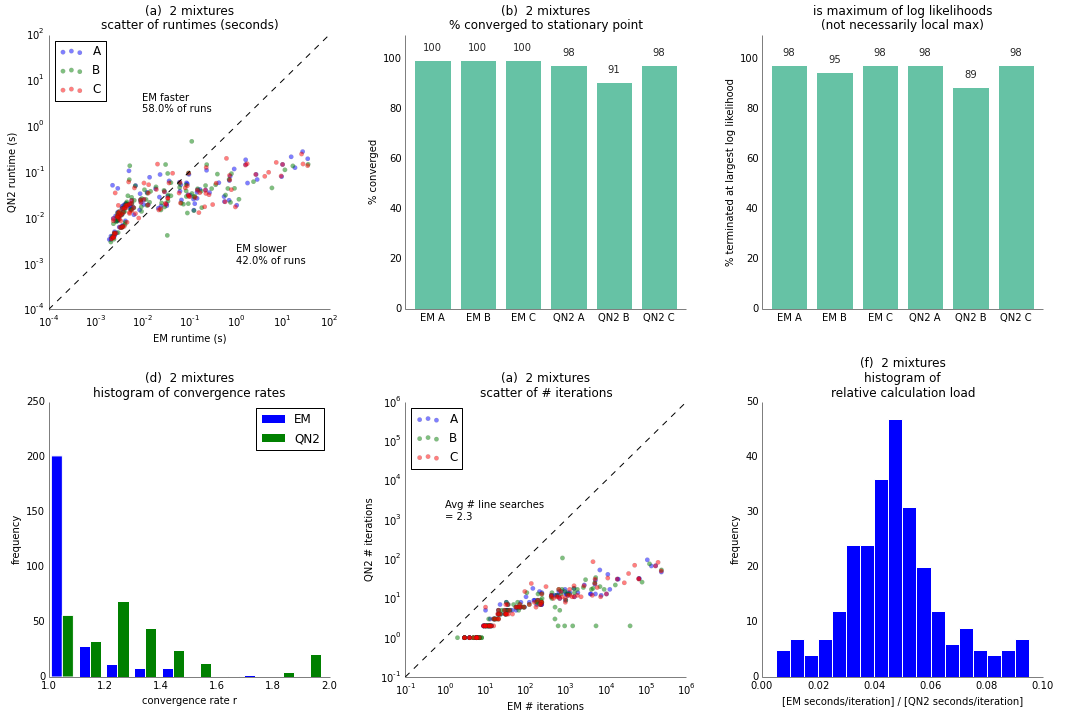
\includegraphics[width=16cm]{fig_RunData2_K2_init3.png}
\caption{Results from running EM and QN2 on randomly generated data from poisson mixtures of size 2.  EM and QN2 were tested on a total of 100 randomly generated problems.  EM and QN2 were each run from 3 different starting points, A,B,and C (described in the previous section).}
\end{figure}

Figure 1a shows a scatter plot of the runtimes for each problem, with EM runtimes on the x-axis and QN2 runtimes on the y-axis.  The color scale refers to the initialization points A, B, and C.  Points below the dotted line correspond to problems in which EM took longer than QN2 to terminate.  Note that the runtimes are on a log scale.  

Given EM's reputation for slow convergence and Quasi-Newton's reputation for superlinear convergence, it is surprising to find that, overall, EM tends to finish before QN2.  However, we can see that EM runtimes have a tendency to "explode", corresponding to sublinear convergence, lending credence to EM's reputation.  QN2 runtimes, on the other hand, tend to lie in a much narrower band (roughly between $10^{-2.5}$ and $10^{-1}$ seconds).

Figures 1b measures one aspect of reliability: how often does the algorithm terminate at a stationary point?  Convergence to a stationary point is defined $rg(\theta_k) \leq f_{tol}$, where $rg(\theta_k)$ is the merit function defined Eqn (\ref{eq:rg}).  All EM runs successfully terminated at a stationary point.  Not all of the QN2 runs converged to a stationary point.  QN2 runs that failed to convergence did so because the line search failed.  Recall that as part of the QN2 algorithm, if line search fails, then $S_k$ is reset to $\boldsymbol{0}_{2n \times 2n}$.  If after this reset line search fails again, then QN2 has no more options and consequently breaks and returns an error.  QN2 with initialization B shows the worst performance.  Further work could be done to determine more successful line search strategies for QN2.

Figure 1c measures another aspect of reliability: did the algorithm converge to the largest likelihood?  Here I loosely defined a tolerance range of $10^{-3}$ for comparing one log likelihood function value to another.  Meaning that values with $10^{-3}$ of each other are considered the same.  This threshold seemed to sufficiently capture nearly all of the of the "close" values.  Initialization B shows a lower reliability in both EM and QN2 runs.

Figure 1d plots a histogram of the observed convergence rates of EM and QN2.  Since optimal points are unknown, the convergence rate $r$ at iteration $k$ is loosely defined as:
\[
\frac{|rg(\theta_k+1)|}{|rg(\theta_k)|^r} = 1
\indent
\rightarrow
\indent
r = \frac{\log(rg(\theta_k+1))}{\log(rg(\theta_k))}
\]
The reported convergence rates are the average of the convergence rate in the final 2 iterations for each run.  Convergence rates were not included for runs that terminated without converging.

Figure 1d shows unsurprising results.  EM shows linear convergence and QN2 shows superlinear convergence.

Figure 1e is another scatter plot showing the number of iterations required to terminate.  Each dot represents the EM iterations vs the QN2 iterations for a given problem and given initialization.  This plot shows the same behavior as Figure 1a, although it is clear that more iterations are required for EM on all runs.  The average number of QN2 line searches is 2.3.

The larger number of iterations does not imply longer runtimes.  Figure 1f shows the implied relative calculation load, which is calculated as:
\[
\frac{\text{EM seconds per iteration}}{\text{QN2 seconds per iteration}}
\]

The frequency plot is centered around 0.05, which indicates that, on average, a QN2 iteration takes roughly 20 times longer than an EM iteration.

\pagebreak
\subsection{Results: Size 5 Mixtures}

\begin{figure}[h]
\centering
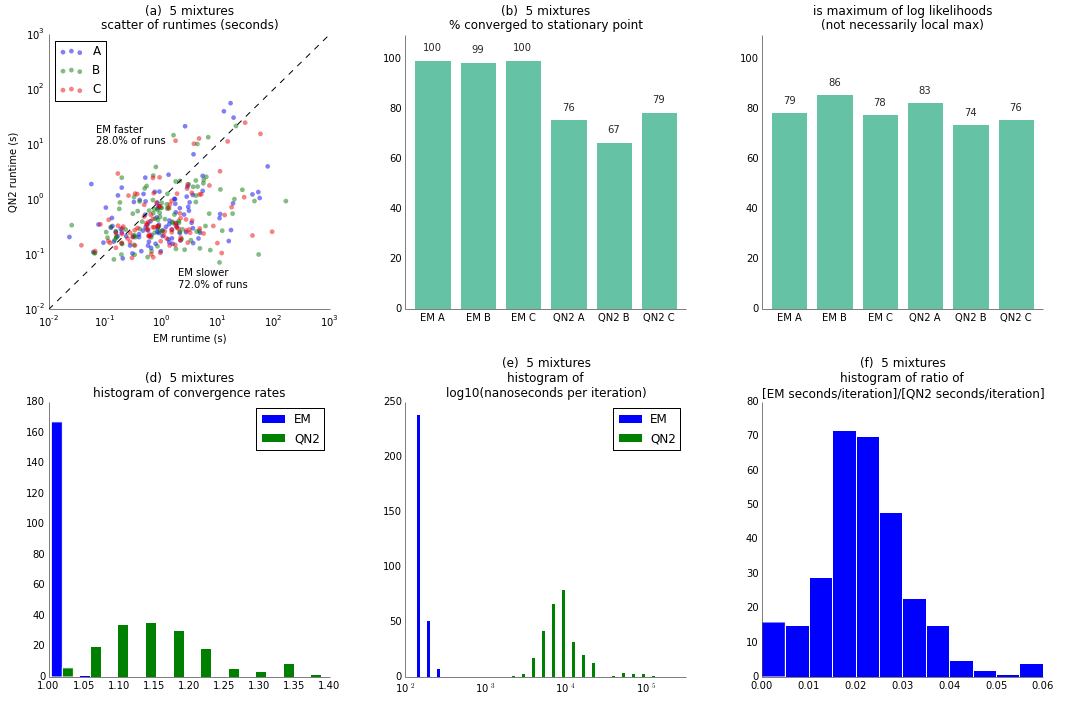
\includegraphics[width=16cm]{fig_RunData2_K5_init3.png}
\caption{Results from running EM and QN2 on randomly generated data from poisson mixtures of size 5.  EM and QN2 were tested on a total of 100 randomly generated problems.  EM and QN2 were each run from 3 different starting points, A,B,and C (described in the previous section).}
\end{figure}

EM shows much slower relative performance in size 5 mixture runs.  Except for 1 one run, all EM runs converged to a stationary point, whereas roughly only 73\% of QN2 terminated at a stationary point.  Again, QN2 initialized on B performed the worst.  The relative calculation load averages at roughly 0.02, meaning approximately 50 EM iterations per 1 QN2 iteration.  This contrasts with the 20:1 ratio seen for size 2 mixtures.  This makes sense given that the number of QN2 line searches has increased dramatically from 2.3 to 141.

\pagebreak
\subsection{Results:  Size 10 Mixtures}
\begin{figure}[h]
\centering
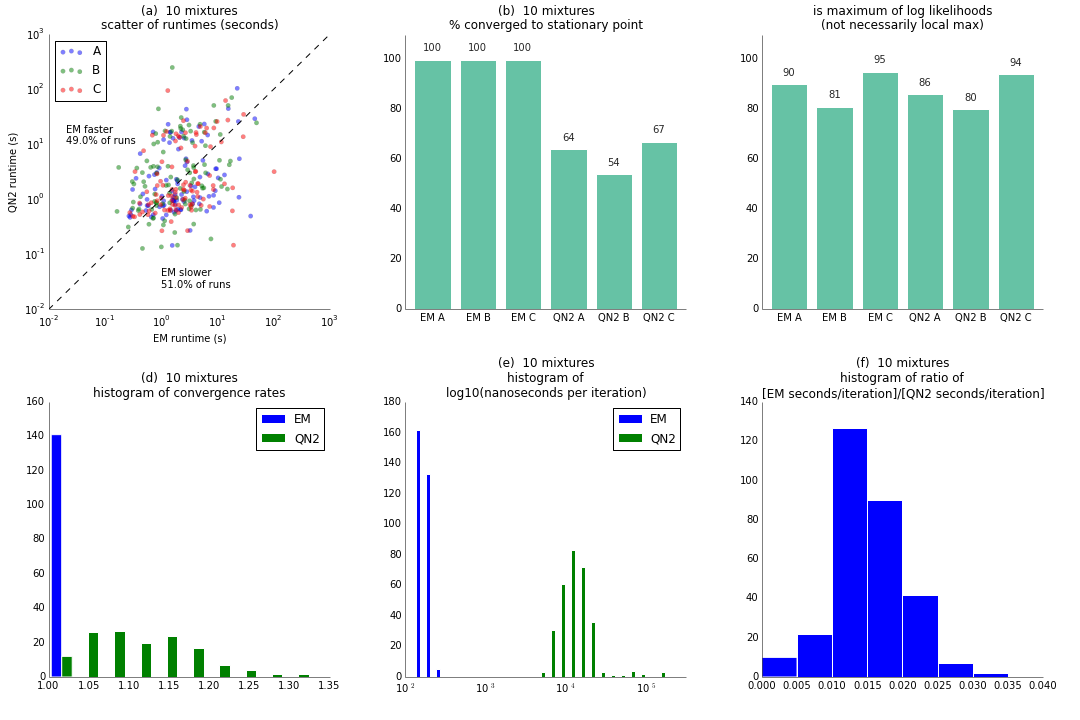
\includegraphics[width=16cm]{fig_RunData2_K10_init3.png}
\caption{Results from running EM and QN2 on randomly generated data from poisson mixtures of size 10.  EM and QN2 were tested on a total of 100 randomly generated problems.  EM and QN2 were each run from 3 different starting points, A,B,and C (described in the previous section).}
\end{figure}

Here we see that the division in runtimes between EM and QN2 is roughly even.  In fact, the spread in the scattor plot also look much more even than in mixtures of size 2 and 5.  The convergence to stationary point success of EM is again perfect, but that of QN2 has decreased further to approximately 59\%.  The distribution of QN2 convergence rates has also decreased somewhat from that for size 2 mixtures.  The average number of QN2 line searches has increased again to 321.5, which is more than double that seen for size 5 mixtures.  The relative calculation load hovers around 0.015, which implies a 66:1 EM iterations to QN2 iterations ratio.

\subsection{Discussion}

Two themes arise from these results.  EM shows little difference in performance across mixture sizes.  QN2 shows worsening performance.

The reason for QN2's worsening performance lies in the number of line searches required.  This is seen in a couple of ways.  First is the increase in convergence failures.  Second is the relative calculation load.  Further work could be done to find better line search strategies. 

As expected, EM showed linear/sublinear convergence and QN2 showed superlinear convergence.  As discussed in sections \ref{section:convergence} and \ref{section:qn2convergence}, given my current understanding and knowledge of the mixture of Poissons likelihood function, not much can be said about convergence to the a local maximizer.  Furthermore, Figures 1c, 2c, and 3c show that convergence to the global maximizer is not guaranteed, and is dependent on algorithm selection and initialization.

In summary, the expected speed improvements of QN2 come with a catch.


\pagebreak
\bibliographystyle{plainnat}
\bibliography{references.bib}
\end{document}
